\begin{comment}
-- Algorithm
 - 1. Pre-processing
	i) Raw data
	
	ii) Filtering, Normalization
	-- Savitzky-Golay Filter and Normalization

	iii) Delta Dirac Functions
	  -- Dictionary Generation
	  -- Dictionary as Dirac Deltas Functions
	  -- Hyperfine Lines
	  -- Independent words
	
	iv) Detection of Lines
	  -- Detection of Candidate Lines: Local Maxima and Minima
	  -- Threshold Detection
	  -- Gaussian Subtraction
	
	v) Recalibration
	Recalibration. Need of Exact Match for Sparse Coding
		a) Exponential Kernel
			Flexibility of the Solution: Gaussian Kernel
		b) Intensity Weight
			Including temperature: Weight

 - 2. Classification
	  -- Lambda Parameter
	  -- Alpha Constraints
	  -- Pseudo-Code
	  
-- Training Set/Tests
	  -- Specifications of Data Cubes
	  -- Different Bands and Variable/Fixed Widths
	  -- Modified Confusion Matrix
\end{comment}

% Algorithm
\section{Algorithm} \label{sec:algorithm}

\begin{figure*}
	\begin{center}
		% 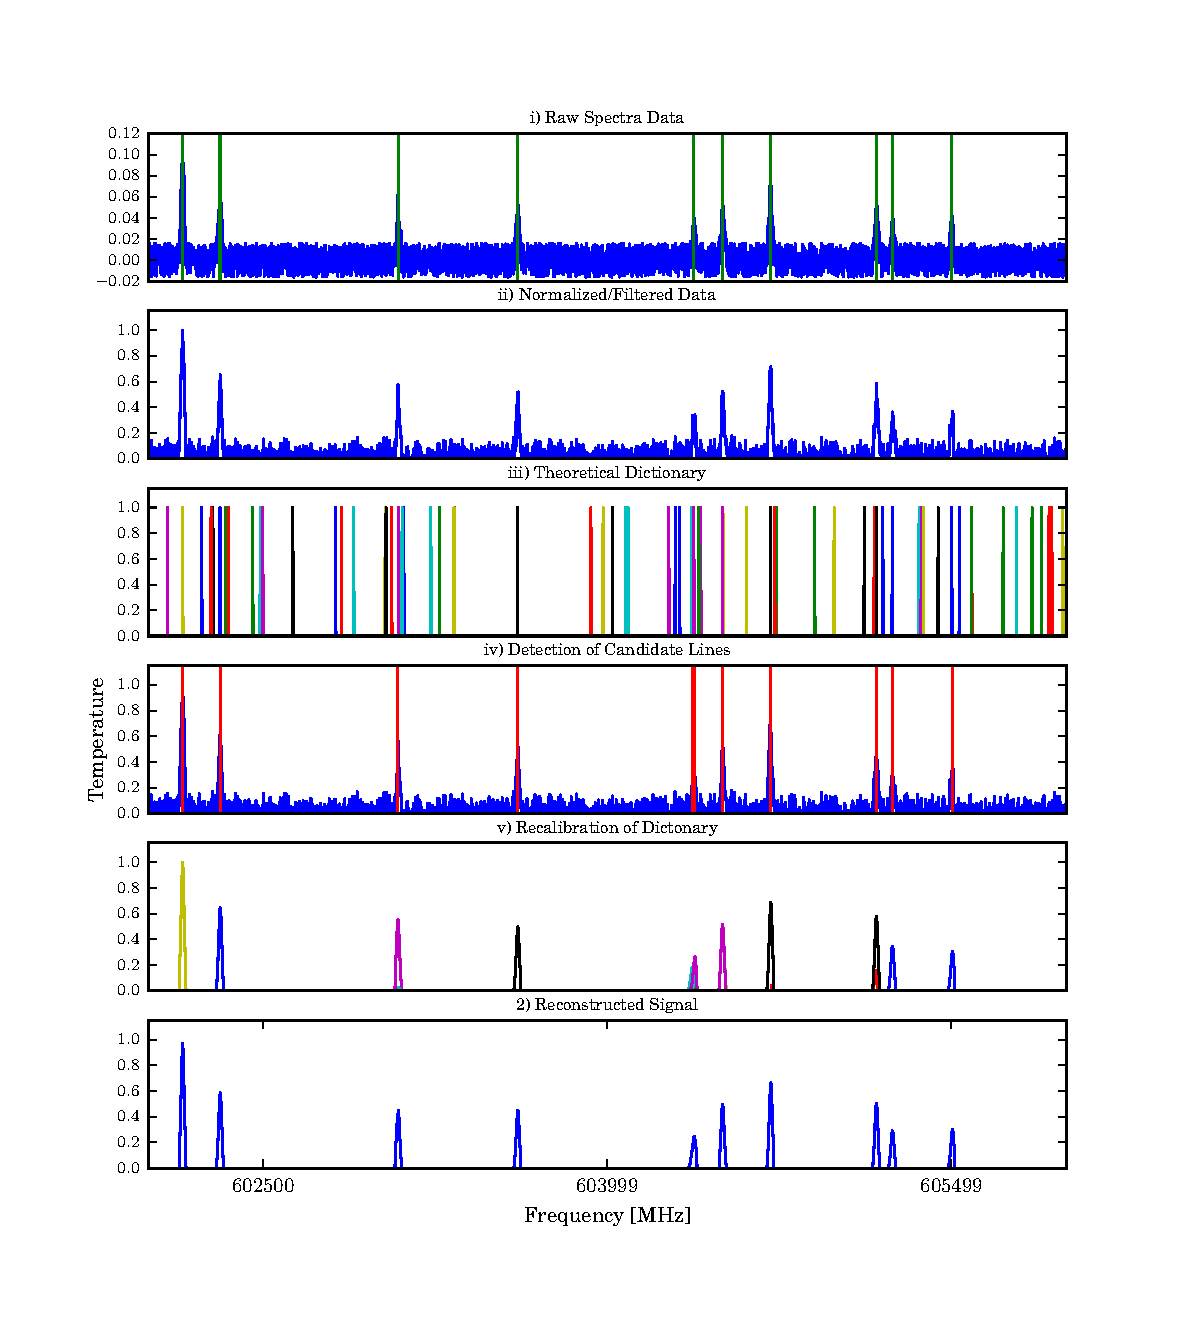
\includegraphics[width=\textwidth]{images/process}
		\label{fig:process}
		\subfigure[]{
			\label{fig:a}
			\clipbox*{0 {.786\height} {1\width} {.9055\height} }{%
				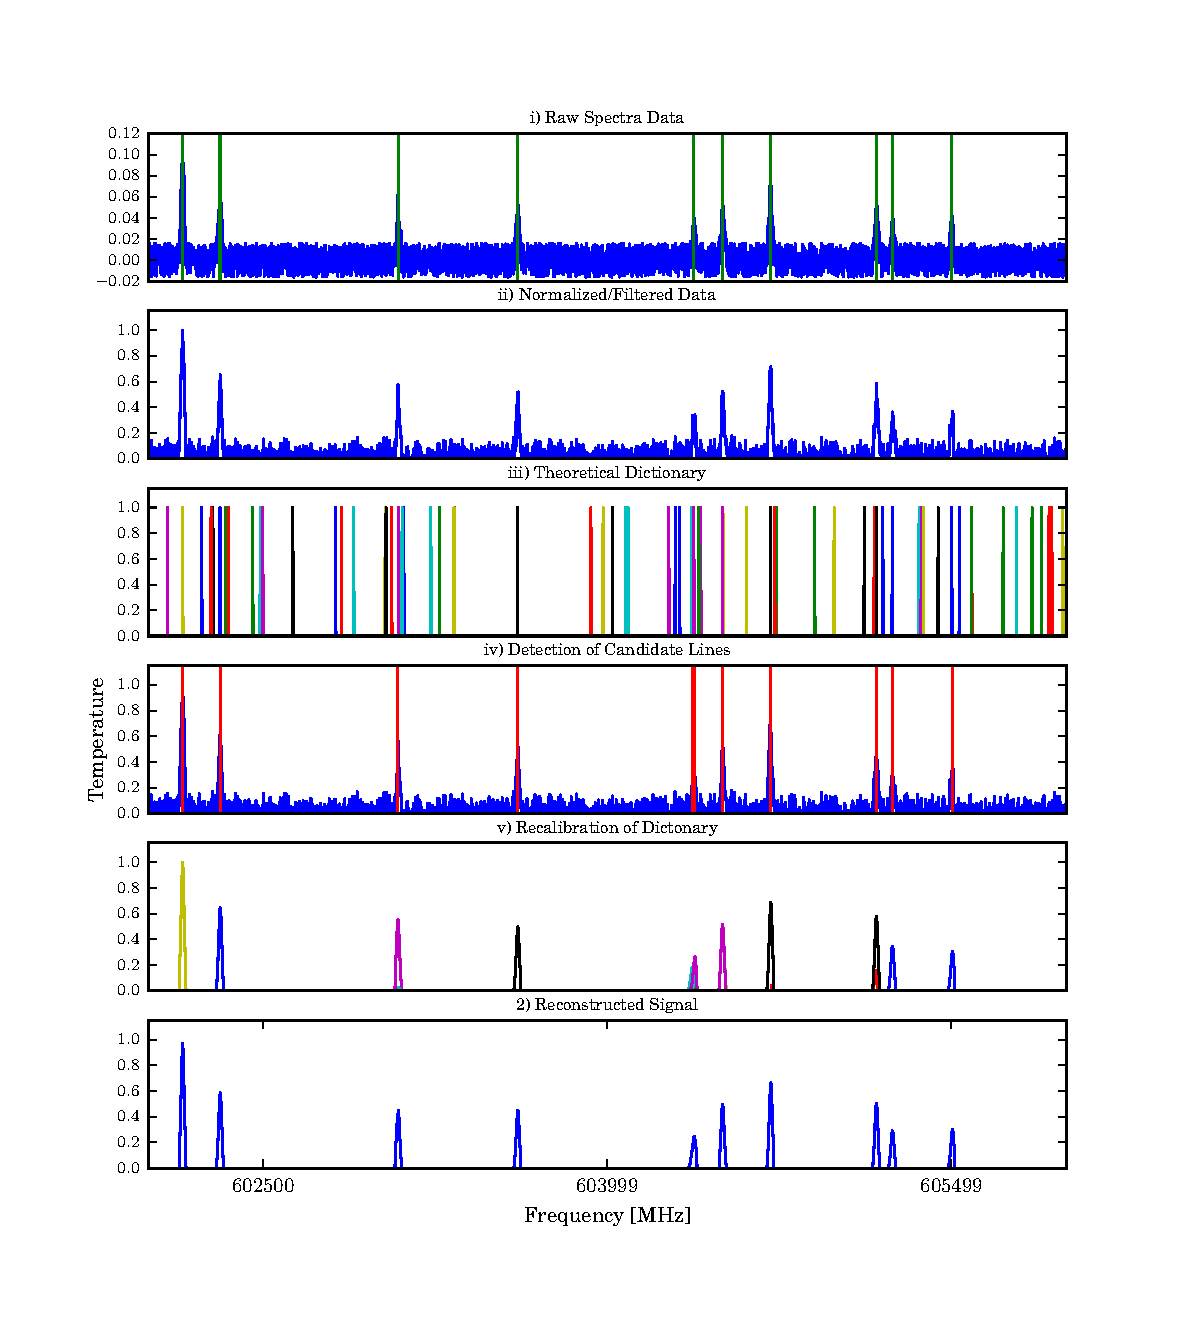
\includegraphics[width=\textwidth,height=450px]{images/process}%
			}%
		}
		\subfigure[]{
			\label{fig:b}
			\clipbox*{0 {.653\height} {1\width} {.770\height} }{%
				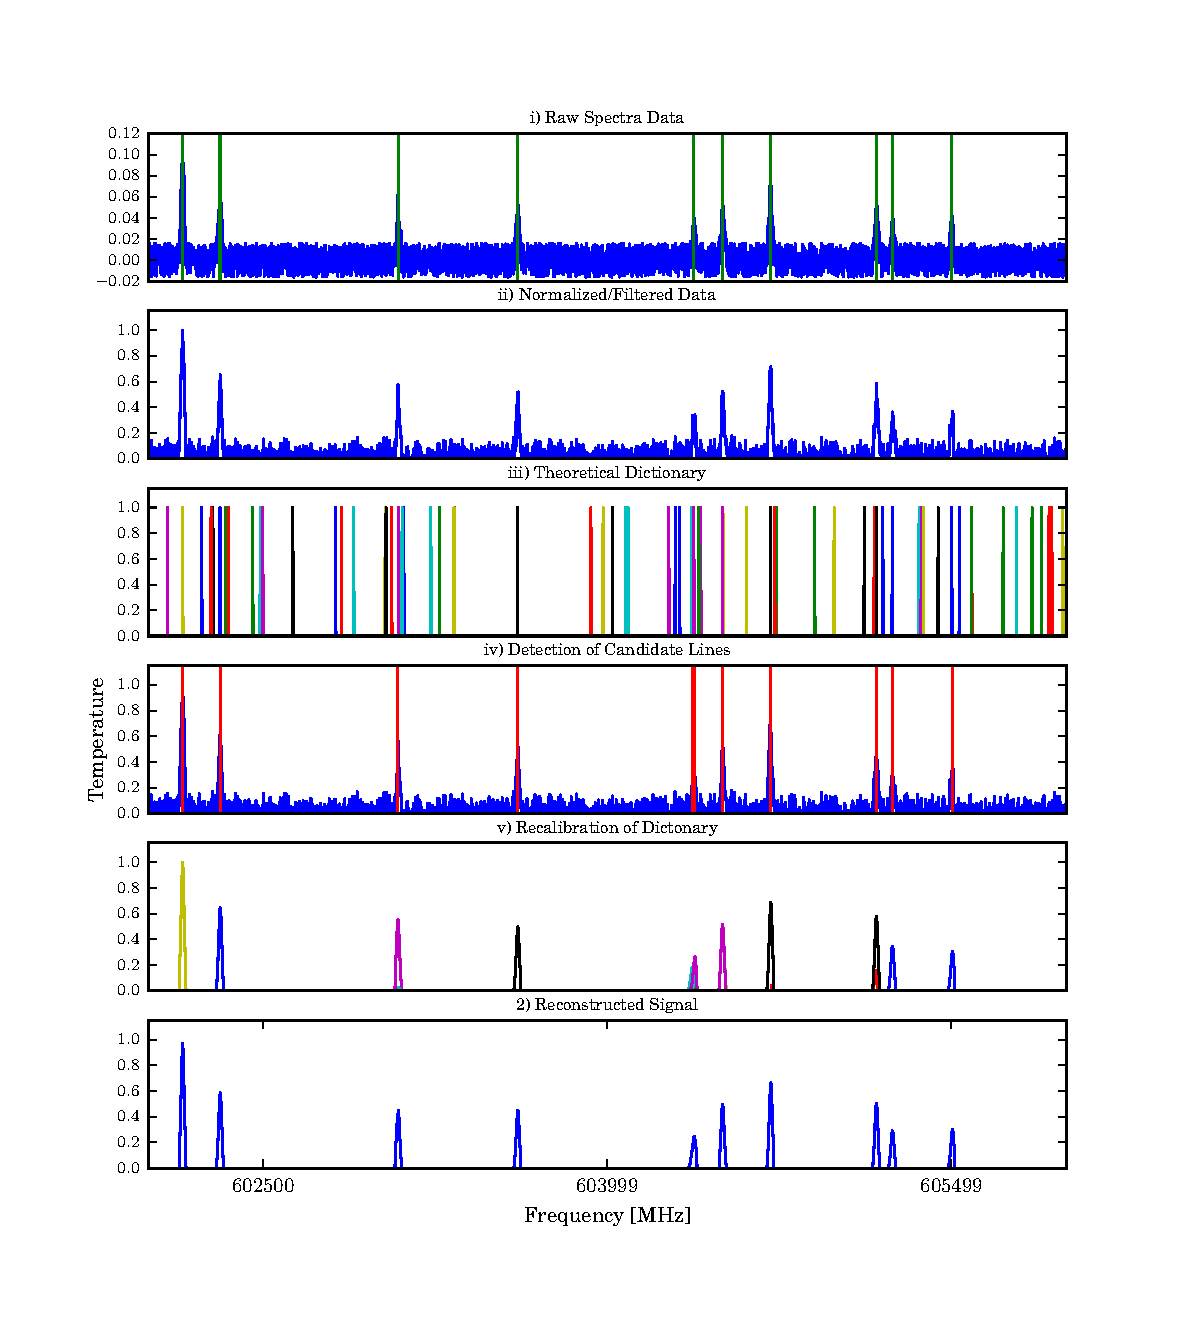
\includegraphics[width=\textwidth,height=450px]{images/process}%
			}%
		}
		\subfigure[]{
			\label{fig:c}
			\clipbox*{0 {.520\height} {1\width} {.640\height} }{%
				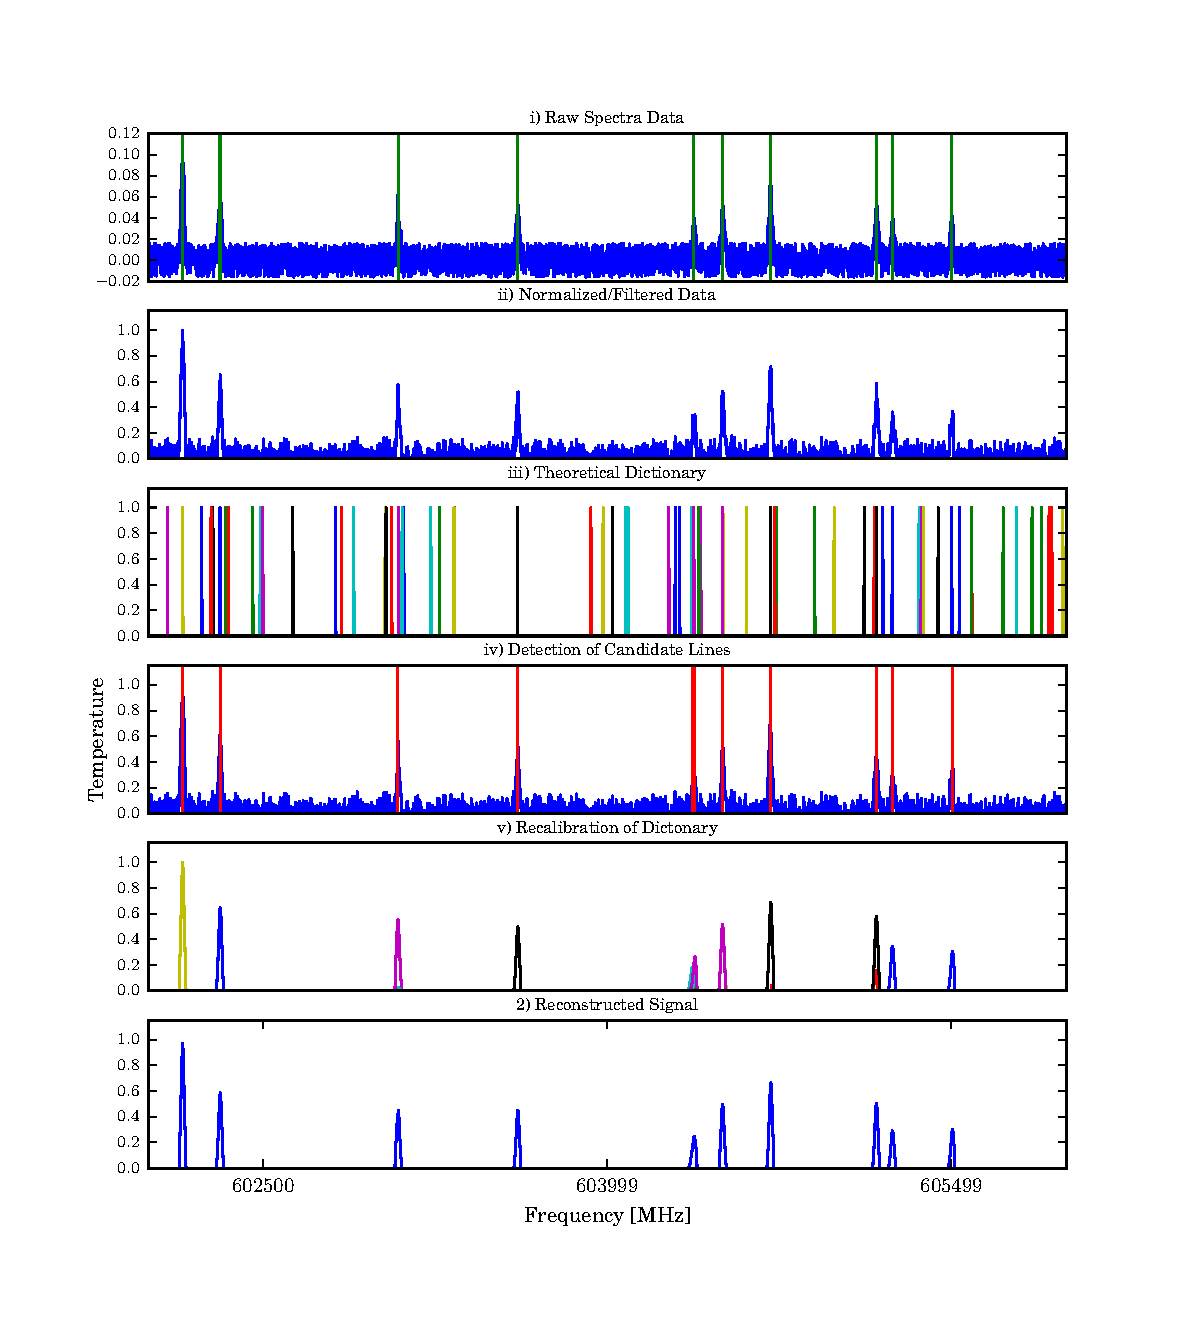
\includegraphics[width=\textwidth,height=450px]{images/process}%
			}%
		}
		\par\medskip
		\subfigure[]{
			\label{fig:d}
			\clipbox*{0 {.387\height} {1\width} {.505\height} }{%
				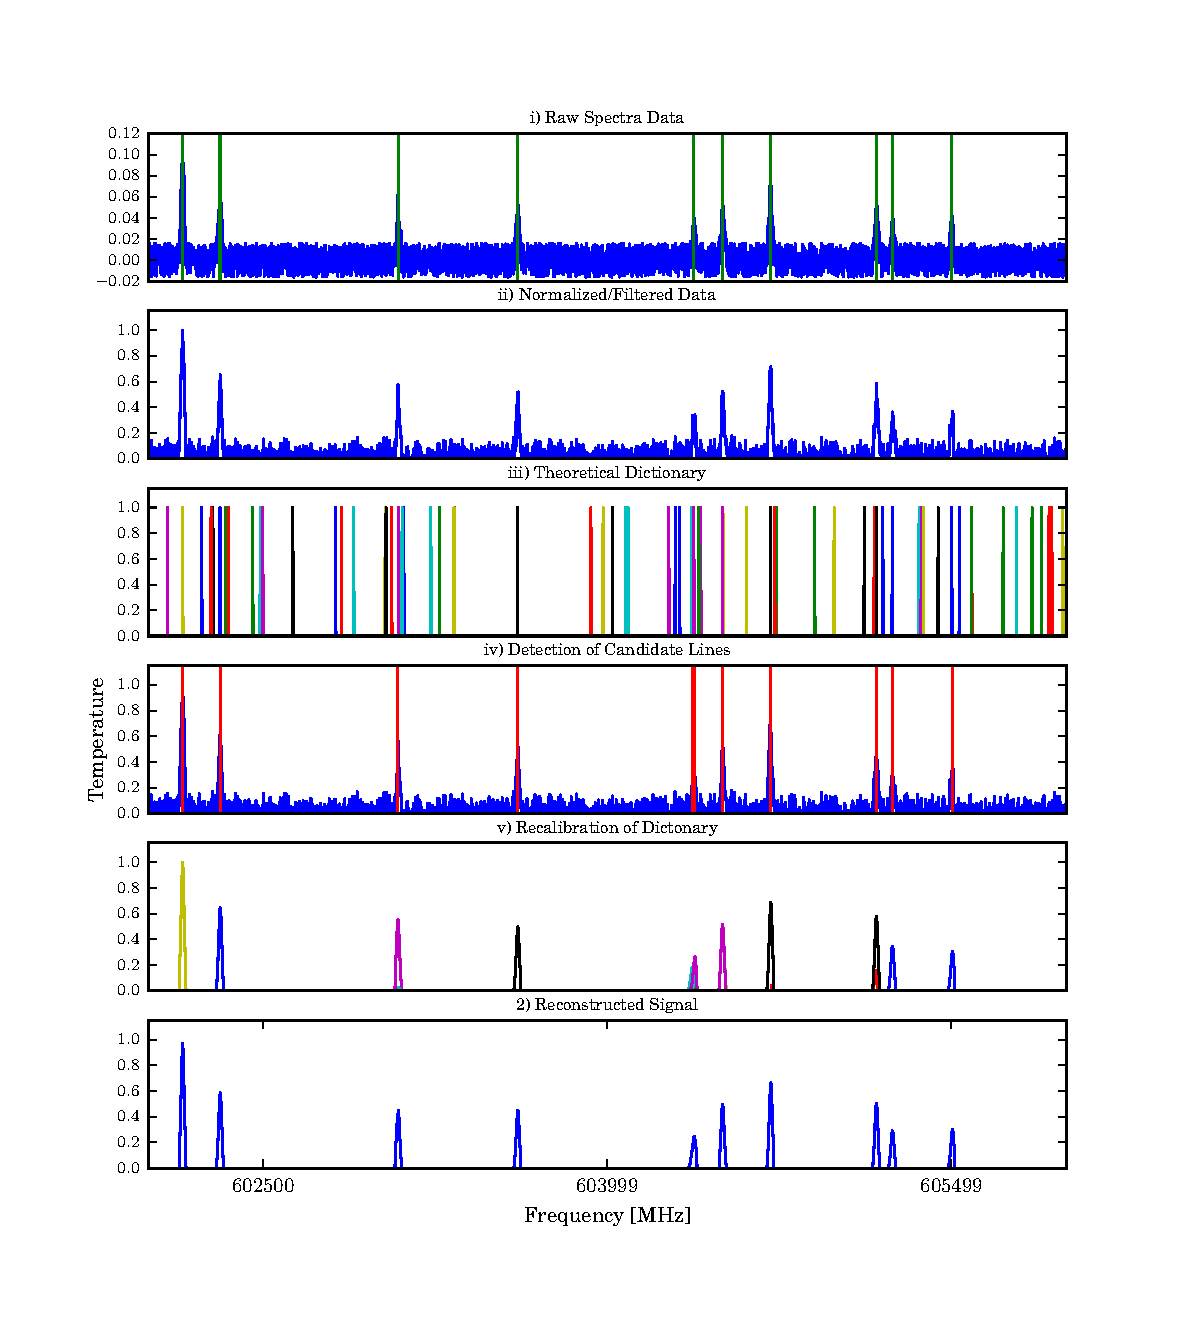
\includegraphics[width=\textwidth,height=450px]{images/process}%
			}%
		}
		\subfigure[]{
			\label{fig:e}
			\clipbox*{0 {.254\height} {1\width} {.370\height} }{%
				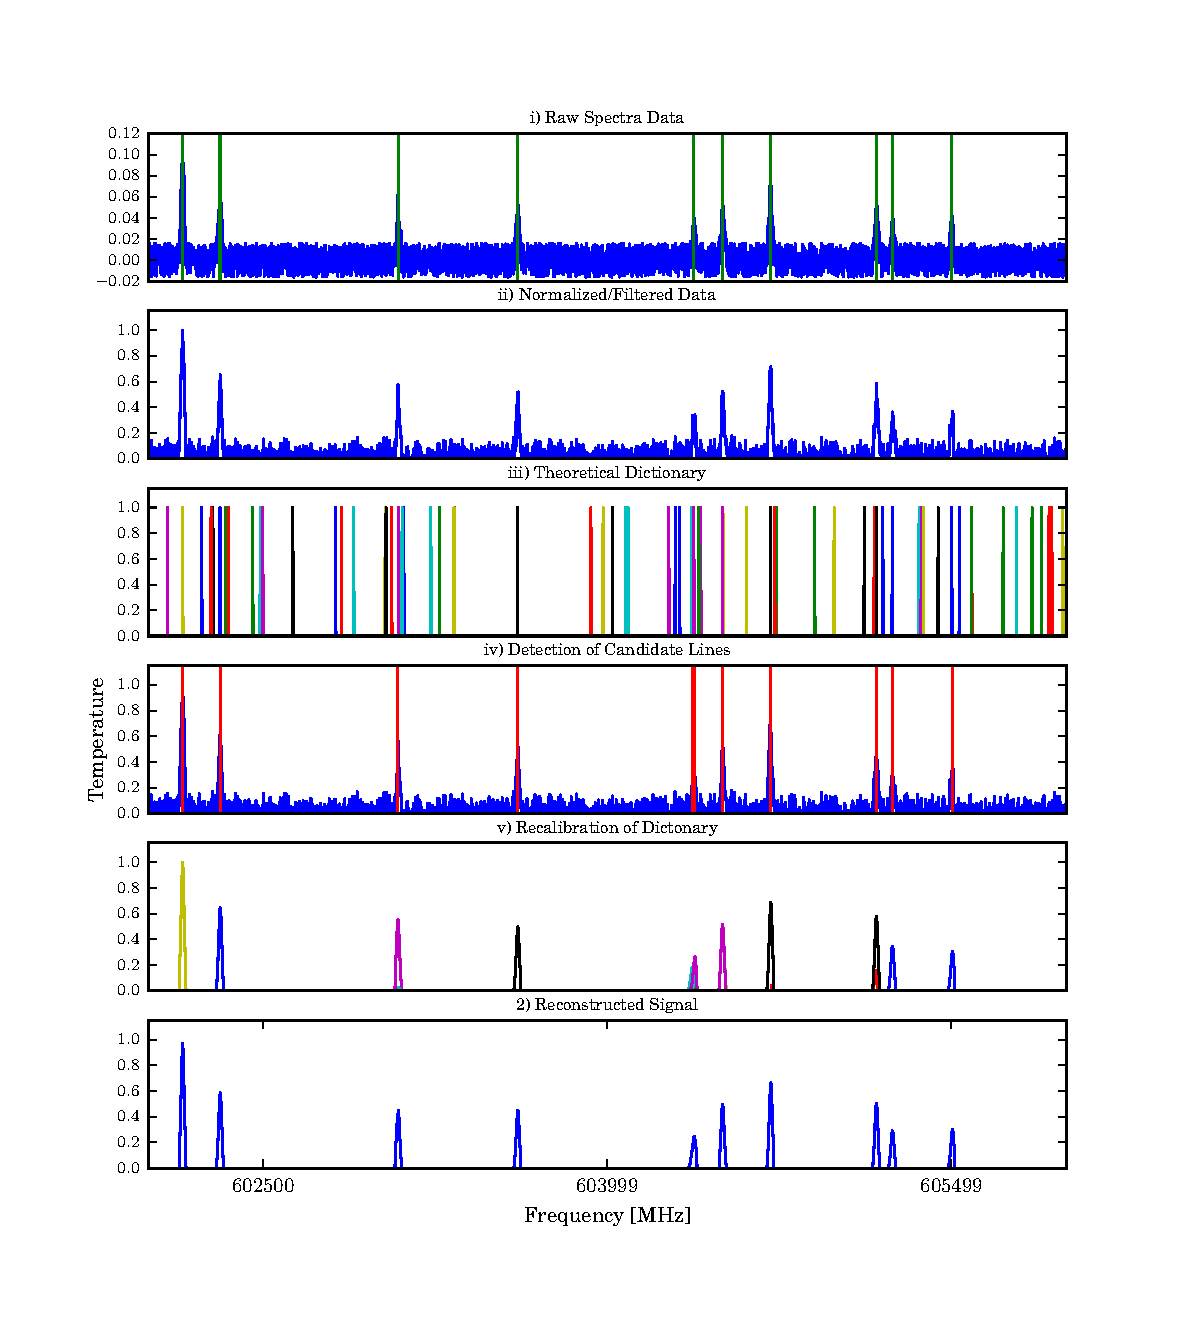
\includegraphics[width=\textwidth,height=450px]{images/process}%
			}%
		}
		\subfigure[]{
			\label{fig:f}
			\clipbox*{0 {.08\height} {1\width} {.240\height} }{%
				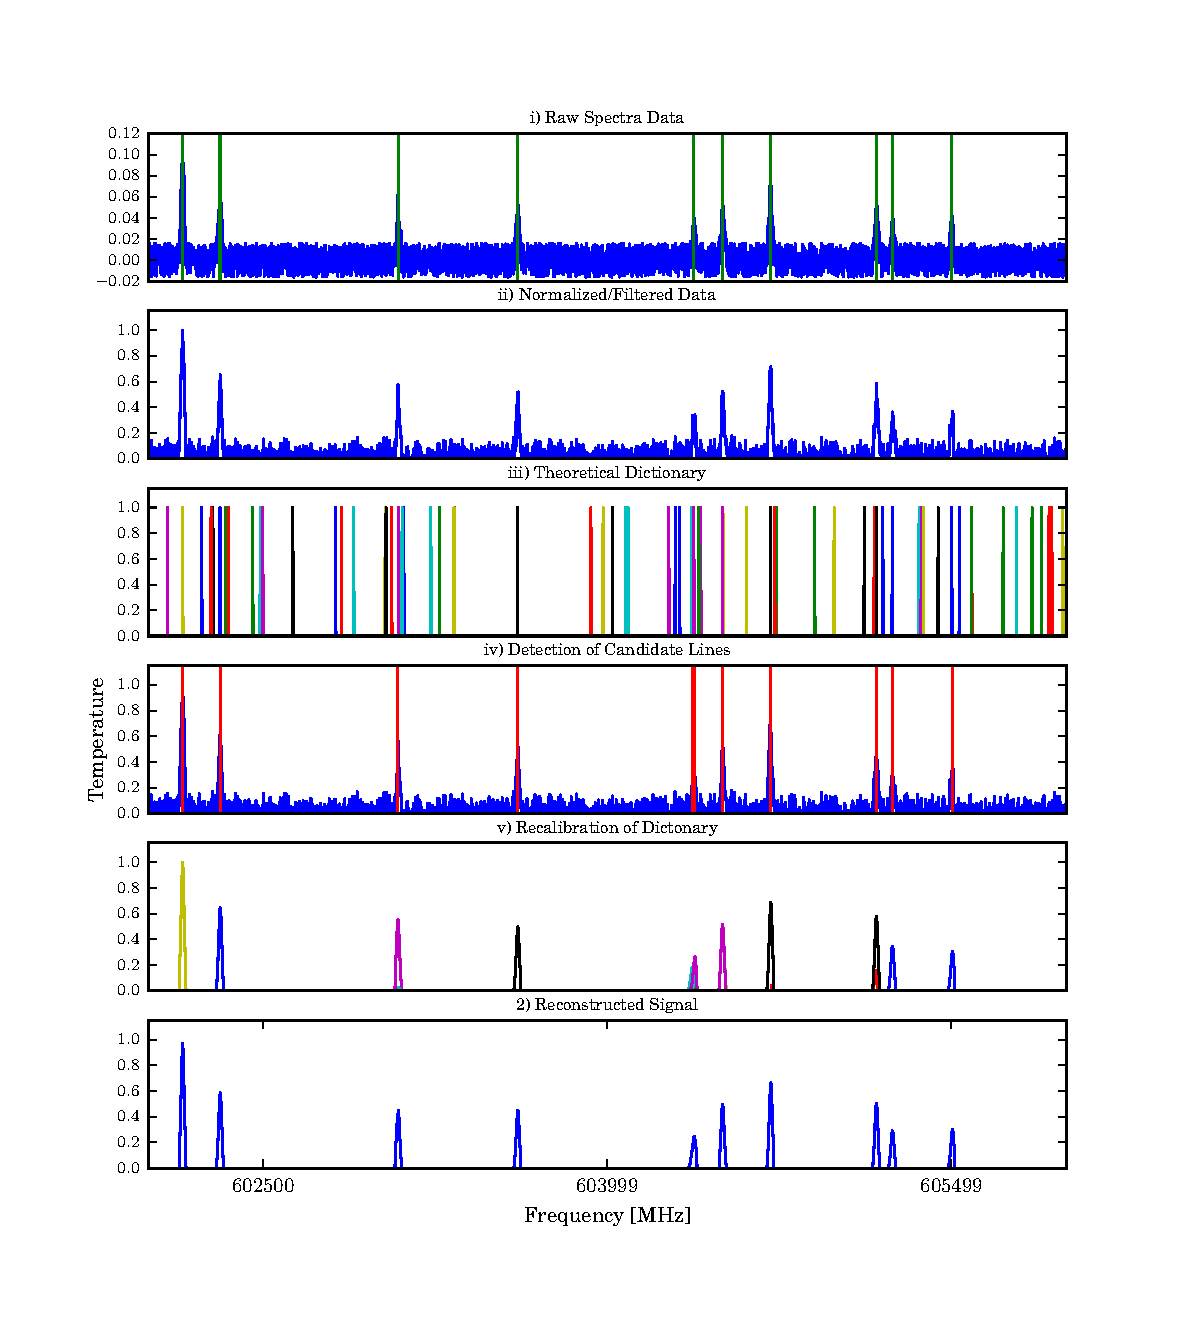
\includegraphics[width=\textwidth,height=450px]{images/process}%
			}%
		}
		\caption{Spectra example though the whole process. Each step: 1. Pre-processing: (a) Read raw data cube, (b) Filter and normalize, (c) Determine dictionary, (d) Detected candidate lines, (e) Recalibrate the dictionary. 2. (f) Reconstruction of the signal.}
	\end{center}
\end{figure*}

Our algorithm has two main steps:
i) spectra pre-processing, which also involves the creation and recalibration of the dictionary, covered in section \ref{sec:preprocessing}.
ii) optimization of equation \ref{eq:sparse_coding}, which allow us later to predict emission lines present along the spectra, viewed at detail in section \ref{sec:prediction}.
An overview of the process is illustrated in figure \ref{fig:process}.

% Pre-processing
\subsection{Pre-processing}  \label{sec:preprocessing}

At first, a dimensional pixel from a data cube is selected to analyze its wavelength range, as shown in figure \ref{fig:a}.
Then, a normalization and filtering of spectra is performed.
Savitzky-Golay filter is applied to reduce white noise influence along the signal\citep{howley_effect_2005}.
Normalization does not have any effects in the sparse coding solution, however, it is applied for convenient purposes, as we will explain later.
Figure \ref{fig:b} illustrates the output after the preprocessing step.

% Dictionary as Dirac Deltas Functions
\subsubsection{Delta Dirac function}
In this stage, we perform the following steps: 
i) select all theoretical lines for all isotopes present in range of measurement.
ii) create delta Dirac vectors for each theoretical line previously selected.
Delta direct functions allow to determine a representative and meaningful dictionary for this problem.
One word is defined for each theoretical frequency known in spectra wavelength range.
This formulation allows to represent each theoretical frequency range with a specific word in the dictionary.

Let $D = \{ w_1, w_2, \ldots, w_d \}$ be the dictionary, where $w_i = [w_{i1}, \ldots, w_{in} ]$ and $w_{ik} \in [0,1] \; \forall i \in [1, \ldots, d] \; \forall k \in [1, \ldots, n]$.
Let $F = \{ f_1, f_2, \ldots, f_n \}$ be the set of frequencies at the range of measure.
The value of each element of $w_i$ is given by the function:

\begin{equation}
	 w_{in} =
	 \begin{cases}
	  1,& \text{if } f_i \text{ is the theoretical frequency of isotope } i\\
	  0,              & \text{otherwise}
	 \end{cases}
	 \label{eq:delta_dirac}
\end{equation}

Figure \ref{fig:c} lists all the theoretical frequencies combined along the spectra in range of measure.

Hyperfine lines are a particular case, in which two close theoretical lines that belong to same isotope are present. In general they are both present as one wider line (see figure \ref{fig:87_77_13C3}).

\begin{figure}[H]
	\begin{center}
		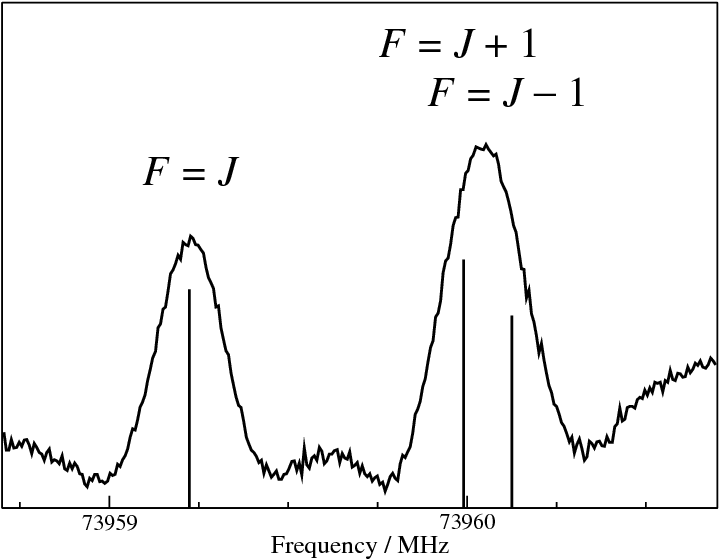
\includegraphics[width=0.35\textwidth]{images/87-77_13C3}
		\caption{Rotational spectrum of vinyl cyanide transition of H$_2^{13}$C=CH−C≡N showing hyperfine unseparable structures \citep{muller_rotational_2008}.}
		\label{fig:87_77_13C3}
	\end{center}
\end{figure}

To deal with hyperfine lines, we combine their delta Dirac functions and merge them into a single word.
Sensitivity of data determines when two hyperfine lines should merge as one.
As we use 1 MHz for sensitivity, two words are merged if they are closer that 1 MHz and belong to the same isotope.

A problem with the use of Dirac Delta functions is that observed lines must be at the precise observed frequencies to be used.
If a difference between a delta Dirac function and its observed candidate line exists, it is impossible for the sparse coding optimization to use the theoretical word to reconstruct the shifted observed frequency.
This makes necessary to adjust the previous words, so that a soft matching can be possible.
If a word is not at the exact frequency than a candidate line's frequency, but near it, the word still can be used, but with a loss of confidence.

Two steps are necessary to make this adjustment to the dictionary: 
i) detect all the candidate lines along the observed spectra, 
ii) expand each word in the recalibration step.

% Detection of Candidate Lines: Local Maxima and Minima
\subsubsection{Candidate emission lines}
We use an heuristic to pre-define frequency ranges at which further steps evaluate the presence or non-presence of emission lines.
A peak detection function is ran to select these ranges associated to possible lines along the spectra. We call these ranges candidate emission lines.

% Threshold Detection
We make use of a threshold given by the 3-$\sigma$ criterion.
An empty pixel is selected from a spectra of the data cube in which the observed object is not present, so that just background and noise is observable.
Then, we compute the mean and standard deviation of the noise.
With this, we search for intensity differences between each consecutive pair of frequencies, and when the difference between the temperature of a frequency and the previous temperature is higher that the threshold, the frequency from higher temperature is saved as candidate line.

% Gaussian Subtraction
Following this idea, an iterative process is performed.
All the peaks are detected from the original spectra and the frequency of the higher intensity is saved as a candidate emission line.
Then, a Gaussian function is fitted at the detected frequency and subtracted from the signal. The process is repeated until the higher intensity of the detected peaks is less than the  3-$\sigma$ threshold.
At the end of the process, a list of candidate lines is determined, as can be seen in figure \ref{fig:d}.

% Recalibration. Need of Exact Match for Sparse Coding
\subsubsection{Recalibration}

% Flexibility of the Solution: Gaussian Kernel
At the end of pre-processing step, the dictionary passes for a step of recalibration, where each word is expanded to a range from the initial Dirac delta function.
We use an exponential kernel function that assign values to each word depending on the distance between theoretical frequencies of the words and their nearest candidate lines.
Word's expansion allows to associate probabilities to matches, which are also used to combine several words at certain frequencies and to replicate blended lines.

In recalibration step, we introduce the use of candidate line's temperature to weight words according to the intensity of the nearest candidate lines.
This reflects that smaller candidate lines are less probable to be emission lines as they get closer in intensity to the threshold.
The final value of a word is given by equation \ref{eq:expansion}.

Let $s = [s_1, s_2, \ldots, s_n]$ be a normalized signal, where $s_i \in [0, 1] \; \forall i \in [1, \ldots, n]$.
Let $D = \{ w_1, w_2, \ldots, w_d \}$ be the dictionary, where $w_i = [w_{i1}, \ldots, w_{in} ]$ and $w_{ik} \in [0,1] \; \forall i \in [1, \ldots, d] \; \forall k \in [1, \ldots, n]$.
Let $F = \{ f_1, f_2, \ldots, f_n \}$ be the set of frequencies at the range of measure. 
Function $c(f)$ is defined as $c(f_i) = s_i, \forall i \in [1, \ldots, n]$, i. e., signal's intensity at frequency $f_i$.
$g$ is defined in \ref{eq:closer_candidate} as the closer candidate line's frequency to a given frequency $f_i$, such as for a word $w_{ki}$:

\begin{equation}
	\label{eq:closer_candidate}
	\begin{aligned}
		\text{$ g $}
		= 
		\text{argmin}
		& _{f} ||f_i - f|| \\
	\end{aligned}
\end{equation}

and a word's expansion is given by equation \ref{eq:expansion}
\begin{equation}
	\begin{aligned}
	\text{$ w_{ki} $}
	= \text{$ c{(g)} $} \cdot \frac{1}{\sqrt{2\pi\sigma}}e^{-\frac{1}{2} (\frac{||f_i - g ||) ^2}{\sigma}}
	\label{eq:expansion}
	\end{aligned}
\end{equation}

For simplicity sake, this case uses $\sigma$ value as 1 that works well in the ALMA domain we analyzed. 

The final representation of the dictionary can be seen in figure \ref{fig:e}. The majority of the words are expanded to low values and only words closer to candidate lines have appreciable values.
    
 
\subsection{Prediction} \label{sec:prediction}
The optimization of equation \ref{eq:sparse_coding} gives a set of convenient alpha values to reconstruct the observed spectra at ranges of interest.
After the reconstruction, at each frequency along the reconstructed spectra, a subset of used words can be obtained.
Alpha values different than zero are used to assign possible isotopes to each detected line. 

% Lambda Parameter
Sparse coding select the minimal amount of alpha values different than zero, so that combined reconstruct the normalized signal.
This amount of non-zero values is restricted by the Lambda sparsity-inducing parameter, which is experimentally determined as the number of detected candidate lines.
This makes sparse coding to use a similar number of words as candidate lines were detected.

% Alpha Constraints
% Alpha > 0 -> Not absorption lines
An important restriction must be applied to the alpha values.
At the convenient solution of the optimization formulation, non-zero values must be positive to be able to detect emission lines, preventing the use of both negative and positive words.
If not, the word's meaning as presence of emission lines would be lost, resulting in over fitting and false positive predictions.

\subsubsection{Probability of prediction}
At candidate line's frequencies, all non-zero alphas that are near to those frequency are used to determine a probability list. The superposition of words is used to deal with blending or false double peaks cases.

Spectra normalization is a convenient convention to give a meaning to alpha values scooped at range $(0,1)$.
If its value is near to 1, its word is used unscaled, and it has an higher probability to be describing candidate lines.
If an alpha value is closer to 0 or has a value higher than 1, to make use of its word is harder for the optimization. 
A symmetric convention allows to assign the same importance to alpha values bellow and over 1.
Let $\alpha = [ \alpha_1, \ldots,  \alpha_d] \; \forall i \in [1, \ldots, d] \;$ be the set of coefficient values for each theoretical isotope state.
\begin{equation}
\alpha^{*}_{k}\text{ = }
\begin{cases}
\alpha_{k},& \text{if } \alpha_{k} \le 1\\
1/\alpha_{k}, & \text{if } \alpha_{k} > 1
\end{cases}
\label{eq:alpha}
\end{equation}

Alphas at each frequency, and its subsequent normalization (by the sum of all alphas used in that frequency), give a probability distribution over possible isotopes.
The probability of presence for theoretical line $k$, at a given frequency $i$, for $D$ isotope states, is given by \ref{eq:probability} 

\begin{equation}
P_{ik} = \cfrac{\alpha^{*}_k}{\sum_{j=1}^{d} \alpha^{*}_j}
\label{eq:probability}
\end{equation}

% Pseudo-Code
The pseudo-code of the algorithm is summarized in \ref{alg:algorithm}.

\begin{algorithm}[H]
    \KwData{$data\_cube$, $isotopes\_set$}
        \KwResult{$probability\_predictions$}
            get parameters from $data\_cube$\;
            get input spectra from pixel of $data\_cube$\;
            compute $threshold$ from noise\;
            get $Dictionary$ from $isotopes\_set$\;
            initialize $candidate\_set$ as $[(\;)]$\;
            detect $max\_set$ from spectra\;
            $max_{freq} = max(max\_set)$\;
            \While{$(max_{freq} > threshold)$}{
                ($candidate\_set$).append($max_{freq}$)\;
                subtract Gaussian function at $max_{freq}$\;
	            detect $max\_set$ from residual spectra\;
	            $max_{freq} = max(max\_set)$\;
            }
            recalibrate $Dictionary$ from $candidate\_set$\;
            get $alphas$ from solving sparse coding\;
            compute $probability\_predictions$ from $alphas$\;
            return $probability\_predictions$\;
    \caption{Proposed algorithm}
   	\label{alg:algorithm}
\end{algorithm}


% Specifications of Data Cubes
\subsection{Training/Test set}
For testing purposes, each lines present in simulated spectras are stored as data cube meta-data, allowing us to evaluate the predictive model and determine metrics to validate predictions.

% How we separated the data
Because of ALMA measurements and ASYDO simulator capabilities, we yield specifications for data cube with two main distinctions:
i) signal to noise ratio, using different ALMA bands
ii) fixed/variable width of lines, 
% Different Bands and Variable/Fixed Widths
% Different Band (Noise)
For i), the differences lie in both signal to noise ratio and spectral line density.
ALMA bands 7 and 9 are selected for experiments, and the test consists in 50 cubes, in which half of them are run for different subsets of isotopes present at both ranges 602 - 606 $GHz$ (ALMA band 9) and 275 - 277 $GHz$ (ALMA band 7).
For ii), 50 test run on the same bands, but using variable line width.
Each line width is assigned independently in a range of variation of $(-2, +2) MHz$ from original width.


